
\documentclass[handout,8pt]{beamer}
\usepackage{framed}
\usepackage{geometry}
\usetheme{metropolis}
\usepackage{tikz}
\usetikzlibrary{shadows}
\geometry{paperwidth=9.5cm,paperheight=6.8cm}
\setbeamertemplate{navigation symbols}{}
\setbeamertemplate{frametitle}[default][center]
\setbeamersize{text margin left=15pt,text margin right=15pt}
\usefonttheme{serif}
\setbeamerfont{frametitle}{size=\Huge}
\definecolor{codegreen}{rgb}{0,0.6,0}
\definecolor{codered}{rgb}{0.6,0,0}
\newenvironment{greenframe}{%
	\setbeamercolor{frametitle}{bg=codegreen}
	\begin{frame}
	}{%
	\end{frame}
}
\setbeamercolor{frametitle}{bg=codered}
\usepackage{graphicx}
\usepackage[most]{tcolorbox}
\setbeamertemplate{navigation symbols}{}
\setbeamertemplate{frametitle}{%
	\nointerlineskip%
	\begin{beamercolorbox}[wd=\paperwidth,ht=2.5ex,dp=1.5ex]{frametitle}
		\centering
		\hspace*{1ex}\insertframetitle%
	\end{beamercolorbox}%
}
\hyphenation{Accepto}
\begin{document}

\begin{frame}[plain]{Reviewer 2}
    \begin{columns}
        \begin{column}{0.5\textwidth}
            \centering
            \tikz\node[inner sep=0pt, draw=none, drop shadow={shadow xshift=1mm,shadow yshift=-1mm,fill=black, opacity=0.3}]{
                
\includegraphics[width=\linewidth]{images/br_role_1}
            };
        \end{column}
        \begin{column}{0.5\textwidth}
            \begin{tcolorbox}[left=2pt,right=2pt,colback=white,colframe=codered,fonttitle=\bfseries, title=Reviewer 2]
                An academic legend who's never met a paper he liked. His feedback always begins with \textbf{`I enjoyed reading this, however,'} followed by countless critiques. If you are lucky, you get a \textbf{`Weak Reject'}. Rumor has it, if your rejection didn't make you cry, you didn't get Reviewer 2.
            \end{tcolorbox}
        \end{column}
    \end{columns}
\end{frame}

\begin{frame}[plain]{Rejecting Reviewer}
    \begin{columns}
        \begin{column}{0.5\textwidth}
            \centering
            \tikz\node[inner sep=0pt, draw=none, drop shadow={shadow xshift=1mm,shadow yshift=-1mm,fill=black, opacity=0.3}]{
                
\includegraphics[width=\linewidth]{images/br_role_2}
            };
        \end{column}
        \begin{column}{0.5\textwidth}
            \begin{tcolorbox}[left=2pt,right=2pt,colback=white,colframe=codered,fonttitle=\bfseries, title=Doktor Schon Gehört]
                Doktor Schon Gehört always has a nostalgic air about him, endlessly droning on about old academic papers nobody else recalls. Like a broken record, he can't resist pointing out, \textbf{`Schon gehört!'}, as if the world of research began and ended with him.
            \end{tcolorbox}
        \end{column}
    \end{columns}
\end{frame}

\begin{frame}[plain]{Rejecting Reviewer}
    \begin{columns}
        \begin{column}{0.5\textwidth}
            \centering
            \tikz\node[inner sep=0pt, draw=none, drop shadow={shadow xshift=1mm,shadow yshift=-1mm,fill=black, opacity=0.3}]{
                
\includegraphics[width=\linewidth]{images/br_role_3}
            };
        \end{column}
        \begin{column}{0.5\textwidth}
            \begin{tcolorbox}[left=2pt,right=2pt,colback=white,colframe=codered,fonttitle=\bfseries, title=Herr Überflieger]
                Herr Überflieger has quite the reputation. He's known for this \textbf{`bird's-eye view'}, often saying, `I've read enough to judge.' Sadly, `enough' is rarely more than the title.
            \end{tcolorbox}
        \end{column}
    \end{columns}
\end{frame}

\begin{frame}[plain]{Rejecting Reviewer}
    \begin{columns}
        \begin{column}{0.5\textwidth}
            \centering
            \tikz\node[inner sep=0pt, draw=none, drop shadow={shadow xshift=1mm,shadow yshift=-1mm,fill=black, opacity=0.3}]{
                
\includegraphics[width=\linewidth]{images/br_role_4}
            };
        \end{column}
        \begin{column}{0.5\textwidth}
            \begin{tcolorbox}[left=2pt,right=2pt,colback=white,colframe=codered,fonttitle=\bfseries, title=Dr. Curry Critique]
                Dr. Curry Critique likens papers to spice blends. Always hunting for academic \textbf{`zing'}, he always comments, \textbf{`Needs more masala, doesn't it?'} when dismissing a paper.
            \end{tcolorbox}
        \end{column}
    \end{columns}
\end{frame}

\begin{frame}[plain]{Rejecting Reviewer}
    \begin{columns}
        \begin{column}{0.5\textwidth}
            \centering
            \tikz\node[inner sep=0pt, draw=none, drop shadow={shadow xshift=1mm,shadow yshift=-1mm,fill=black, opacity=0.3}]{
                
\includegraphics[width=\linewidth]{images/br_role_5}
            };
        \end{column}
        \begin{column}{0.5\textwidth}
            \begin{tcolorbox}[left=2pt,right=2pt,colback=white,colframe=codered,fonttitle=\bfseries, title=Ms. Bollywood Drama]
                A product of Bollywood's script writing schools, Ms.~Bollywood Drama seeks theatrics even in academia. To her, a paper isn't merely a collection of facts; it's an epic awaiting a dramatic twist. Boring submissions often earn her critique, \textbf{`Needs more drama!'}.
            \end{tcolorbox}
        \end{column}
    \end{columns}
\end{frame}

\begin{frame}[plain]{Rejecting Reviewer}
    \begin{columns}
        \begin{column}{0.5\textwidth}
            \centering
            \tikz\node[inner sep=0pt, draw=none, drop shadow={shadow xshift=1mm,shadow yshift=-1mm,fill=black, opacity=0.3}]{
                
\includegraphics[width=\linewidth]{images/br_role_6}
            };
        \end{column}
        \begin{column}{0.5\textwidth}
            \begin{tcolorbox}[left=2pt,right=2pt,colback=white,colframe=codered,fonttitle=\bfseries, title=Space King]
                Space King can detect a misplaced space from a mile away. For him, even the best research fades if the letters aren't breathing right. \textbf{`Spacing's off. Start over,'} he declares, not bothering to read past the title.
            \end{tcolorbox}
        \end{column}
    \end{columns}
\end{frame}

\begin{frame}[plain]{Rejecting Reviewer}
    \begin{columns}
        \begin{column}{0.5\textwidth}
            \centering
            \tikz\node[inner sep=0pt, draw=none, drop shadow={shadow xshift=1mm,shadow yshift=-1mm,fill=black, opacity=0.3}]{
                
\includegraphics[width=\linewidth]{images/br_role_7}
            };
        \end{column}
        \begin{column}{0.5\textwidth}
            \begin{tcolorbox}[left=2pt,right=2pt,colback=white,colframe=codered,fonttitle=\bfseries, title=Madam Nicht Gut]
                Madam Nicht Gut is the epitome of rigorous academic critique. With every paper she reviews, she looks for that impeccable harmony of thought, akin to the perfect aesthetic. When it is incoherent, she screams \textbf{`Das~ist~nicht~gut!'}
            \end{tcolorbox}
        \end{column}
    \end{columns}
\end{frame}

\begin{frame}[plain]{Rejecting Reviewer}
    \begin{columns}
        \begin{column}{0.5\textwidth}
            \centering
            \tikz\node[inner sep=0pt, draw=none, drop shadow={shadow xshift=1mm,shadow yshift=-1mm,fill=black, opacity=0.3}]{
                
\includegraphics[width=\linewidth]{images/br_role_8}
            };
        \end{column}
        \begin{column}{0.5\textwidth}
            \begin{tcolorbox}[left=2pt,right=2pt,colback=white,colframe=codered,fonttitle=\bfseries, title=Prof. Ivory Tower]
                Prof. Ivory Tower is the epitome of academic elitism. Living in his ivy-covered tower, he's rumored to have not set foot in the `real world' for decades. Every paper is a mere layman's work. His critiques often start with, \textbf{`In~my vast experience...'} and end with a predictable rejection.
            \end{tcolorbox}
        \end{column}
    \end{columns}
\end{frame}

\begin{greenframe}[plain]{Accepting Reviewer}
    \begin{columns}
        \begin{column}{0.5\textwidth}
            \centering
            \tikz\node[inner sep=0pt, draw=none, drop shadow={shadow xshift=1mm,shadow yshift=-1mm,fill=black, opacity=0.3}]{
                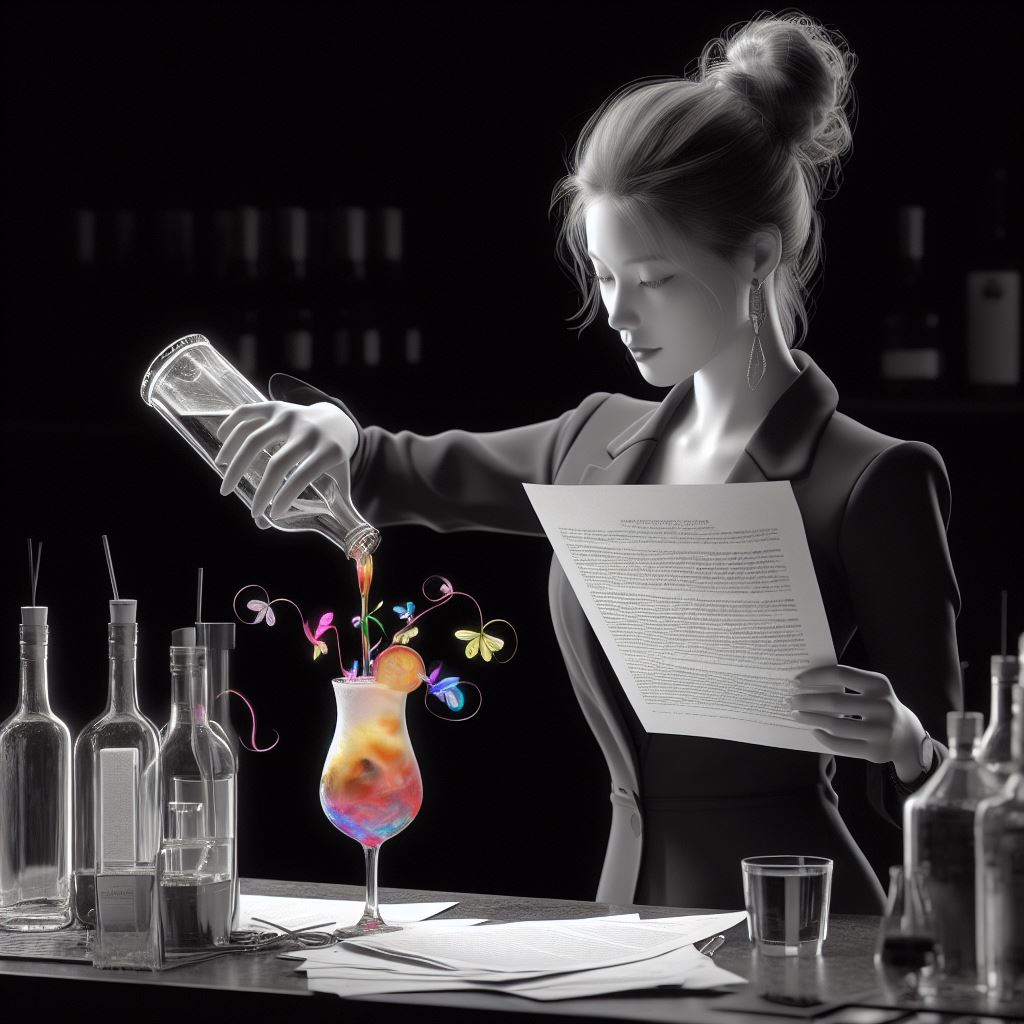
\includegraphics[width=\linewidth]{images/gr_role_1}
            };
        \end{column}
        \begin{column}{0.5\textwidth}
            \begin{tcolorbox}[left=2pt,right=2pt,colback=white,colframe=codegreen,fonttitle=\bfseries, title=Mixmaster Maddy]
                Maddy, a bartender-researcher, considers every paper a cocktail of ideas. She believes in blending theories smoothly. \textbf{`Stir in a strong conclusion like a punchy cocktail!'} she advises while pouring a vibrant cocktail. Her reviews are both sharp and intoxicating.
            \end{tcolorbox}
        \end{column}
    \end{columns}
\end{greenframe}

\begin{greenframe}[plain]{Accepting Reviewer}
    \begin{columns}
        \begin{column}{0.5\textwidth}
            \centering
            \tikz\node[inner sep=0pt, draw=none, drop shadow={shadow xshift=1mm,shadow yshift=-1mm,fill=black, opacity=0.3}]{
                
\includegraphics[width=\linewidth]{images/gr_role_2}
            };
        \end{column}
        \begin{column}{0.5\textwidth}
            \begin{tcolorbox}[left=2pt,right=2pt,colback=white,colframe=codegreen,fonttitle=\bfseries, title=Magical Meera]
                Meera wields a wand and a pen with equal flair. For her, every paper carries its own magic, even if hidden. \textbf{\textit{`Accepto Manuscripto!'}} she chants, making every fault disappear, accepting papers with her wand.
            \end{tcolorbox}
        \end{column}
    \end{columns}
\end{greenframe}

\begin{greenframe}[plain]{Accepting Reviewer}
    \begin{columns}
        \begin{column}{0.5\textwidth}
            \centering
            \tikz\node[inner sep=0pt, draw=none, drop shadow={shadow xshift=1mm,shadow yshift=-1mm,fill=black, opacity=0.3}]{
                
\includegraphics[width=\linewidth]{images/gr_role_3}
            };
        \end{column}
        \begin{column}{0.5\textwidth}
            \begin{tcolorbox}[left=2pt,right=2pt,colback=white,colframe=codegreen,fonttitle=\bfseries, title=Kebab King]
                The döner maestro, this man doesn't just wrap kebabs, he wraps praise and critiques together seamlessly. \textbf{`Such fiery research needs--salate alles und alles drei soße!'} he often suggests. Serving sizzling reviews is his forte, often sandwiched with hearty encouragement.
            \end{tcolorbox}
        \end{column}
    \end{columns}
\end{greenframe}

\begin{greenframe}[plain]{Accepting Reviewer}
    \begin{columns}
        \begin{column}{0.5\textwidth}
            \centering
            \tikz\node[inner sep=0pt, draw=none, drop shadow={shadow xshift=1mm,shadow yshift=-1mm,fill=black, opacity=0.3}]{
                
\includegraphics[width=\linewidth]{images/gr_role_4}
            };
        \end{column}
        \begin{column}{0.5\textwidth}
            \begin{tcolorbox}[left=2pt,right=2pt,colback=white,colframe=codegreen,fonttitle=\bfseries, title=Bavarian Brigitte]
                Brigitte, with her classic Bavarian spirit, resonates with Oktoberfest vibes all year round. For her, every paper deserves a \textbf{`Prost!'}. With braided hair, traditional dirndl, and enthusiasm, she often says, \textbf{`More of this, and the academic world will dance in joy!'}
            \end{tcolorbox}
        \end{column}
    \end{columns}
\end{greenframe}

\begin{greenframe}[plain]{Accepting Reviewer}
    \begin{columns}
        \begin{column}{0.5\textwidth}
            \centering
            \tikz\node[inner sep=0pt, draw=none, drop shadow={shadow xshift=1mm,shadow yshift=-1mm,fill=black, opacity=0.3}]{
                
\includegraphics[width=\linewidth]{images/gr_role_5}
            };
        \end{column}
        \begin{column}{0.5\textwidth}
            \begin{tcolorbox}[left=2pt,right=2pt,colback=white,colframe=codegreen,fonttitle=\bfseries, title=Libori Louis]
                Louis, Paderborn's pride, is as festive in his reviews as the city during Libori. He celebrates the spirit of Libori not just once a year, but with every review. \textbf{`This paper? A reason to celebrate!'} he proclaims, handing out constructive praise like Libori sweets.
            \end{tcolorbox}
        \end{column}
    \end{columns}
\end{greenframe}

\begin{greenframe}[plain]{Accepting Reviewer}
    \begin{columns}
        \begin{column}{0.5\textwidth}
            \centering
            \tikz\node[inner sep=0pt, draw=none, drop shadow={shadow xshift=1mm,shadow yshift=-1mm,fill=black, opacity=0.3}]{
                
\includegraphics[width=\linewidth]{images/gr_role_6}
            };
        \end{column}
        \begin{column}{0.5\textwidth}
            \begin{tcolorbox}[left=2pt,right=2pt,colback=white,colframe=codegreen,fonttitle=\bfseries, title=Prof. Barbie]
                With her impeccable fashion sense and a love for all things pink, Prof. Barbie is here to bring style to the academic world. \textbf{`Darling, your paper is absolutely fabulous! It's a total runway hit!'} she gushes, ever so enchanted by the flair and panache of your writing.
            \end{tcolorbox}
        \end{column}
    \end{columns}
\end{greenframe}

\begin{greenframe}[plain]{Accepting Reviewer}
    \begin{columns}
        \begin{column}{0.5\textwidth}
            \centering
            \tikz\node[inner sep=0pt, draw=none, drop shadow={shadow xshift=1mm,shadow yshift=-1mm,fill=black, opacity=0.3}]{
                
\includegraphics[width=\linewidth]{images/gr_role_7}
            };
        \end{column}
        \begin{column}{0.5\textwidth}
            \begin{tcolorbox}[left=2pt,right=2pt,colback=white,colframe=codegreen,fonttitle=\bfseries, title=Guidance Guru]
                Dwelling under the banyan's shade, this Indian guru reads beyond mere words. \textbf{`The cosmic energy of your paper resonates with ancient vibrations,'} he says. He feels every paper should be rooted in old wisdom. \textbf{`Infuse your findings with facts as old as the Vedas'} is his sage advice.
            \end{tcolorbox}
        \end{column}
    \end{columns}
\end{greenframe}

\begin{greenframe}[plain]{Accepting Reviewer}
    \begin{columns}
        \begin{column}{0.5\textwidth}
            \centering
            \tikz\node[inner sep=0pt, draw=none, drop shadow={shadow xshift=1mm,shadow yshift=-1mm,fill=black, opacity=0.3}]{
                
\includegraphics[width=\linewidth]{images/gr_role_8}
            };
        \end{column}
        \begin{column}{0.5\textwidth}
            \begin{tcolorbox}[left=2pt,right=2pt,colback=white,colframe=codegreen,fonttitle=\bfseries, title=Santa Scholar]
                Santa Scholar is known for his jovial approach to reviewing, always bearing gifts of acceptance. He believes every researcher deserves a holiday cheer. While he sees your mistakes, he's too focused on the good you've done. \textbf{`You have been a well-behaved academic! Here's your present: \textit{Acceptance!}'}
            \end{tcolorbox}
        \end{column}
    \end{columns}
\end{greenframe}

\end{document}
